% !TEX ROOT = ../ersti.tex
\newpage\mathphyssecnobar{Lehramt Mathematik}\vspace*{-3em}%FIXME
%\section{Lehramt Mathematik}
\subsection{Allgemeines} Der Lehramtsstudiengang birgt so einige Schwierigkeiten, was aber kein Grund zum Aufgeben sein sollte. Eine der größten Schwierigkeiten in den ersten Semestern ist wohl die Koordination der beiden Fächer. Da sich nicht jede Fakultät mit den anderen abspricht, sind Überschneidungen insbesondere in Anfängervorlesungen die Regel. Gerade die Anfängervorlesungen Analysis und Lineare Algebra werden euch im ersten Jahr recht viel Zeit kosten, sodass es sein kann, dass ihr nicht beide hören könnt und gleichzeitig auch noch das volle Regelprogramm eures zweiten Hauptfaches. Insbesondere bei Kombinationen aus den Naturwissenschaften heraus ist dieser Fall leider eher die Regel. Ihr müsst Euch dann entscheiden, Vorlesungen wegzulassen und auf spätere Semester zu verschieben. Das ist aber nicht schlimm, ihr habt genügend Zeit. Dabei solltet ihr beachten, dass manche Vorlesungen als Orientierungsprüfung zählen, einige Vorlesungen aufeinander aufbauen und  manche Vorlesungen nicht regelmäßig angeboten werden. Fragt am besten nach! Bei solchen Problemen können die Fachstudienberatung, Lehramtskandidaten in höheren Semestern oder natürlich die Fachschaft (meistens) weiterhelfen. Diese Probleme haben  schon andere vor euch gehabt und eine Lösung gefunden.

\subsection{Die Orientierungsprüfung} Die erste Hürde im Studium ist die Orientierungsprüfung,  die in beiden Hauptfächern abgelegt werden muss (eine in Mathematik  und die andere beispielsweise -- so weiß der Teufel -- in Theologie).
% einfügen des orientierungsprüfungsartikels.\\
Die \emph{Orientierungsprüfung} für das Hauptfach Mathematik wird studienbegleitend abgelegt und besteht aus der erfolgreichen Teilnahme am Teilmodul „Lineare Algebra 1“. Spätestens bis nach dem dritten Semester solltet ihr sie bestehen, da ihr andernfalls den Prüfungsanspruch verliert, es sei denn ihr habt die Fristüberschreitung nicht zu vertreten (z.B. aus Krankheitsgründen o.ä.).

\subsection{Grundstudium und Zwischenprüfung}
Das Grundstudium ist der erste Teil des Studiums, in dem ihr die Grundlagen der verschiedenen Teilbereich der Mathematik erlernt und der offiziell mit dem bestehen der Zwischenprüfung endet. Die Zwischenprüfung wird wie die Orientierungsprüfung studienbegleitend abgenommen und besteht aus der erfolgreichen Teilnahme an den Gesamtmodulen Analysis und Lineare Algebra. Ins Grundstudium zählen ferner auch die Einführungsveranstaltungen in die Stochastik und Numerik.

Ihr habt ganze 6 Semester Zeit, um die Zwischenprüfung zu bestehen, wobei die meisten Kommiliton\_innen sie formal zum 3. Semester ablegen.  Man kann natürlich auch vor der Zwischenprüfung Vorlesungen aus dem Hauptstudium hören.

\subsection{Hauptstudium und wissenschaftliche Prüfung}
Das Hauptstudium ist der zweite Teil eures Studiums. Hier vertieft ihr Eure Kenntnisse in Teilbereichen der Mathematik aufbauend auf den Vorkenntnissen des Hauptstudiums. Kursusvorlesungen des Hauptstudiums sind beispielsweise Algebra, Zahlentheorie oder Geometrie. Die Gebiete, in denen ihr euch hier vertieft, werdet ihr auch als Prüfungsgebiete in eurer wissenschaftlichen Prüfung angeben können. Die Wissenschaftliche Prüfung („Staatsexamensprüfung“) bildet den Abschluss des Lehramtsstudiums. Sie wird in der Regel im oder nach dem 10. Semester abgelegt. Sie dauert 60 Minuten und erstreckt sich über den Inhalt von drei Teilgebieten des Hauptstudiums (in der Regel also drei Vorlesungen zu je 4 \gls{SWS}) sowie mathematisches Grundlagen- und Überblickswissen.

\subsection{Wissenschaftliche Arbeit}

Sofern ihr eure wissenschaftliche Arbeit in Mathematik schreiben möchtet, werdet ihr euch in einem der Gebiete des Hauptstudiums noch weiter spezialisieren, um danach in einer der Arbeitsgruppen eine eigene mathematische Facharbeit anzufertigen. In der Regel dauert das circa 4 Monate, wobei je nach Themengebiet durchaus noch eine gewisse Einarbeitungszeit mit berücksichtigt werden muss.


\subsection{Studienaufbau konkret}

Um euch einen Anhaltspunkt für eure Studienplanung zu geben, findet ihr im Folgenden eine Liste der Pflicht-, Wahlpflicht- und Wahlmodule, die ihr insgesamt belegen müsst. Seitens der Fakultät gibt es zusätzlich noch einen Musterstudienplan. Da ihr allerdings nicht umhin kommt, je nach eurem weiteren Hauptfach, eurer Studiensituation (Nebenjob o.ä.) etc. euren Studienverlaufplan selbst zu erstellen, möchten wir den Musterplan an dieser Stelle nicht angeben. Die ersten Semester sind ohnehin dadurch festgelegt, dass i.d.R. nur die Grundvorlesungen ohne weitere Vorkenntnisse besuchbar sind.\\

\vfill
\begin{figure}[h]
\centering{
%    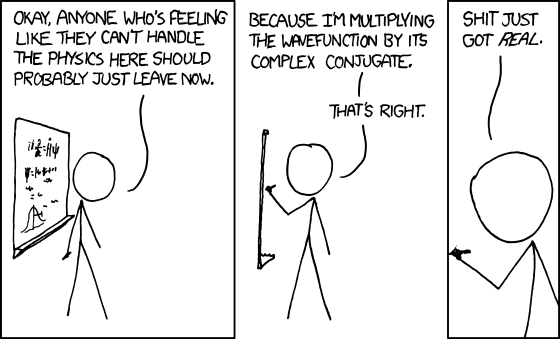
\includegraphics[width=.7\textwidth]{complex_conjugate.png}
    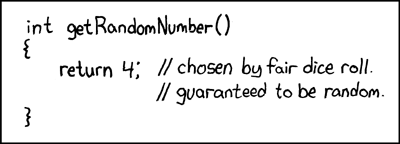
\includegraphics[width=.75\textwidth]{random_number.png}
}
\end{figure}
\vfill
\newpage%FIXME

\begin{tabular}{lc}
  \toprule
  \emph{Grundvorlesungen Pflichtbereich:}\\
  \midrule
  Analysis 1 & 8 LP\\
  Analysis 2 & 8 LP\\
  \addlinespace
  Lineare Algebra 1 & 8 LP\\
  Lineare Algebra 2 & 8 LP\\
  \addlinespace
  Einführung in die Wahrscheinlichkeitstheorie und Statistik & 8 LP\\
  Einführung in die Numerik & 8 LP\\[4mm]

  \emph{Kursusvorlesungen Pflichtbereich:}\\
  \midrule
  Geometrie & 8 LP\\
  Elementare Zahlentheorie & 8 LP\\
  Algebra 1 & 8 LP\footnote{Hinweis: Da diese Vorlesung zum einen in der Regel von der Person gelesen wird, die im Semester zuvor Lineare Algebra 2 gelesen hat, empfiehlt es sich, Algebra 1 direkt im dritten Semester zu hören. Da die Algebra 1 auch diejenige Vorlesung ist, die in eurem Studiengang erfahrungsgemäß die meisten Probleme bereitet, hat dies den zusätzlichen Vorteil, dass ihr recht früh die schwierigste Vorlesung bestanden habt und nicht am Ende eures Studiums evtl. noch den Prüfungsanspruch verliert.}\\
  Funktionentheorie 1 & 8 LP\\[4mm]

  \emph{Wahlpflichtbereich:}\\
  \midrule
  Kursusvorlesung nach Wahl & 8 LP\\
  Seminar nach Wahl & 6 LP\\[4mm]

  \emph{Fachdidaktikbereich:}\\
  \midrule
  Vorlesung & 4 LP\\
  Fachdidaktische Übung & 6 LP\\
  \bottomrule
\end{tabular}
